\definecolor{Purple}{RGB}{153,0,153}
\begin{frame}{Propagación de restricción}
    La verificación hacia adelante propaga información de variables asignadas a no asignadas, 
    pero no provee detección temprana para todos los fallos
    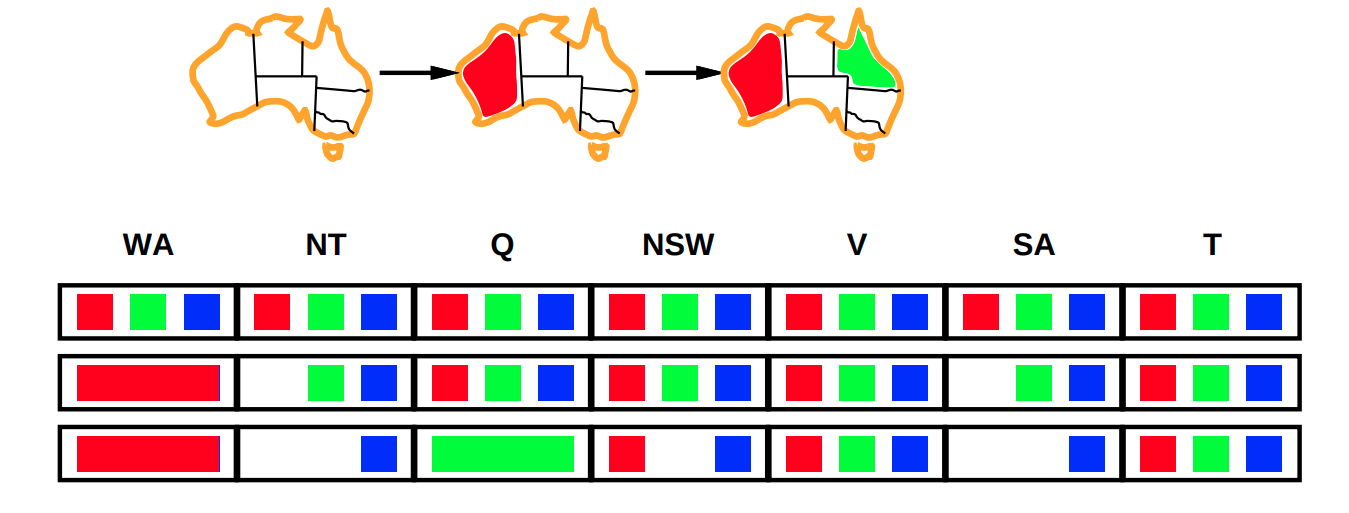
\includegraphics[scale=0.6]{26_image_cap5pag26.png}
    \\
    \textcolor{Purple}{NT} y \textcolor{Purple}{SA} no pueden ser ambos azules
    \\
    \textcolor{blue}{La propagación de restricción} repetidamente reforza localmente las restricciones 
\end{frame}
    